\documentclass[a4paper]{article}           % Switch to report for front page
\usepackage{amsmath,amsfonts,amsthm,amssymb}
\usepackage[utf8]{inputenc}
%\usepackage[icelandic]{babel}
\usepackage[T1]{fontenc}
\usepackage{setspace}                      % Allows more fine-grained control over line spacing
\usepackage{fancyhdr}                      % Headers and footers
\usepackage{lastpage}                      % Allows references to the last page of the document
\usepackage{chngpage}                      % Change format mid-page ?
\usepackage{soul}                          % Highlights text, with \hl{}
\usepackage[usenames,dvipsnames]{color}    % Add color to text
\usepackage{graphicx,float,wrapfig}
\usepackage{ifthen}                        % \ifthenelse{}
\usepackage{listings} 
%\usepackage{courier}                      % Write in a monospace font
%\usepackage{geometry}                      % Because 'fullpage' is outdated
\usepackage{hyperref}
\usepackage[usenames,dvipsnames]{color}
\usepackage{subfig}

\newtheorem{mydef}{Definition}
\newcommand{\Title}{The Arduino as a Hardware Random-Number Generator}
\newcommand{\SubTitle}{Final Report}
\newcommand{\DueDate}{\today} % Or \today
\newcommand{\Class}{Ardrand}
\newcommand{\AuthorClearSpace}{3in}    % How far below the title the author name shoudl appear
\newcommand{\ClassInstructor}{Ýmir Vigfússon}
\newcommand{\AuthorName}{Benedikt Kristinsson}
\newcommand{\DueLang}{}     % Icelandic   (perhaps some ifelse on language pack)
%\newcommand{\DueLang}{Due on}   % English

%\topmargin=-0.45in      
%\evensidemargin=0in     
%\oddsidemargin=0in      
%\textwidth=6.5in        
%\textheight=9.0in       
%\headsep=0.25in         

% This is the color used for comments below
\definecolor{MyDarkGreen}{rgb}{0.0,0.4,0.0}
\definecolor{MyDarkRed}{rgb}{0.4,0.0,0.0}


\lstloadlanguages{Python}
\lstset{language=Python,                        
       %frame=single,                               % Single frame around code
       %basicstyle=\small\ttfamily,                 % Use small true type font
        basicstyle=\small,                          % Don't use ttf
        keywordstyle=[1]\color{Blue}, %\bf          % functions green (bold commented out)
        keywordstyle=[2]\color{Green},              % function arguments purple
        keywordstyle=[3]\color{Red}\underbar,       % User functions underlined and blue
        identifierstyle=,
        commentstyle=\usefont{T1}{pcr}{m}{sl}\color{MyDarkRed}\small,
        stringstyle=\color{MyDarkGreen},              % Strings
        showstringspaces=false,                     % Don't put marks in string spaces
        tabsize=4,
        % To add more keywords
       %morekeywords={},
        % Function parameters
       %morekeywords=[2]{on, off, interp},
        %%% Put user defined functions here
       %morekeywords=[3]{FindESS, homework_example},
        %
       %morecomment=[l][\color{Grey}]{...},        % Line continuation (...) like blue comment
       %numbers=left,                              % Line numbers on left
       %firstnumber=1,                             % Line numbers start with line 1
       %numberstyle=\tiny\color{Grey},             % Line numbers are blue
       %stepnumber=1                               % Line numbers go in steps of 1
        }

% Setup the header and footer
%\pagestyle{fancy} % Pagestyle allows for header/foother
\pagestyle{plain} % No header/footerer
\lhead{\AuthorName}                                                 
\chead{\SubTitle}  
\rhead{\Class}  
%\cfoot{\thepage}   
% \rfoot{Page\ \thepage\ of\ \protect\pageref{LastPage}}
\renewcommand\headrulewidth{0.4pt}                     
%\renewcommand\footrulewidth{0.4pt}                     
% This is used to trace down (pin point) problems in latexing a document:
%\tracingall

%%%%%%%%%%%%%%%%%%%%%%%%%%%%%%%%%%%%%%%%%%%%%%%%%%%%%%%%%%%%%
% Some tools

% Includes a figure
% The first parameter is the label, which is also the name of the figure
%   with or without the extension (e.g., .eps, .fig, .png, .gif, etc.)
%   IF NO EXTENSION IS GIVEN, LaTeX will look for the most appropriate one.
% The second parameter is the width of the figure normalized to column width
%   (e.g. 0.5 for half a column, 0.75 for 75% of the column)
% The third parameter is the caption.
\newcommand{\scalefig}[3]{
  \begin{figure}[ht!]
    % Requires \usepackage{graphicx}
    \centering
    \includegraphics[width=#2\columnwidth]{#1}
    %%% I think \captionwidth (see above) can go away as long as
    %%% \centering is above
    %\captionwidth{#2\columnwidth}%
    \caption{#3}
    \label{#1}
  \end{figure}}

% Includes code
% The first parameter is the label, which also is the name of the script
%   with the file extension the '#1' in the command belove
% The second parameter is the optional caption.
\newcommand{\code}[2]
{\begin{itemize}\item[]\lstinputlisting[caption=#2,label=#1]{#1}\end{itemize}}
  

%\setcounter{secnumdepth}{0}
\newcommand{\problem}[2]
{
   \subsubsection*{\sc{#1}}
               #2
}
\newcommand{\tmpsection}[1]{}
\let\tmpsection=\section

\renewcommand{\section}[2]{

    \ifthenelse{
      \equal{#2}{Heimildir} % I have to be oddly specific here
    }
    {
      \tmpsection{\sc{#1} }
      \tmpsection{\sc{#2} }
    }
    {\tmpsection{\sc{#1} } }
      

}


\title{
    \Class:\ \Title
    \ifthenelse{\equal{\SubTitle}{}}{}{\\{\SubTitle}}
    }
\date{\small{\DueLang\ \DueDate}}
\author{\AuthorName\\Advisor: \ClassInstructor}


\begin{document}
\maketitle

\begin{center}
\textit{For the kid playing space station in the school yard. }
\end{center}

% Uncomment the \tableofcontents and \newpage lines to get a Contents page
% Uncomment the \setcounter line as well if you do NOT want subsections
%       listed in Contents
% Remeber to compile twice
%\setcounter{tocdepth}{1}
%\tableofcontents
%\newpage

%\clearpage
%x\section{Lausn verkefnis og útfærsla}

\begin{abstract}

  Cheap micro-controllers, such as the Arduino or other controllers
  based on the Atmel AVR CPUs, are being deployed in a wide variety of
  projects, ranging from sensors networks to robotic submarines. In
  this paper, we investigate the feasibility of using the Arduino as a
  true random number generator (TRNG). The Arduino Reference Manual
  recommends using it to seed a pseudo random number generator (PRNG)
  due to its ability to read random atmospheric noise from its
  analogue pins. This is an enticing application since true true bits
  of entropy are hard to come by. Unfortunately, we show with
  statistical methods that the atmospheric noise of an Arduino is
  largely predictable in a variety of settings, and is thus a weak
  source of entropy. We explore various methods to extract true
  randomness from the micro-controller and conclude that it should not
  be used in good faith to produce randomness from its analogue pins.

\end{abstract}

\section{Introduction}
% Motivation

So much in our lives may seem random --- so thinking that generating randomness might seem easy at first glance. But when one inquires further one quickly realizes that due to the deterministic nature of CPUs, it is impossible for them to generate random numbers. 

However, there is a great need for unpredictable values in cryptography. Almost all encryption schemes relay on the notion of secret keys so those keys must be generated in a unpredictable way, or else the encryption scheme is useless. Examples of this are the keystream in a one-time-pad, the primes in the RSA algorithm and the challenges used in a challenge-response system\cite{menezes1996,anthes2011}.t

Many secure encryption protocols use nonces (numbers used once) to add ``noise'' in messages\cite{anthes2011}. If these numbers are predictable, the nonces do not serve much purpose. Micro-controllers like the Arduino are heavily used in e.g. sensor networks\cite{tsense} where data integrity is a key issue. It follows that the demand for high quality entropy is rather high in those situations. 

Since regular computers are unable to produce truly random numbers, psuedorandom number generators (denoted PRNG) are mostly used. A PRNG is a one-way function $f$ the generates random sequnces, of either integers or bits, from an intial seed $s$ and then applies the function iteratively to generate the sequcene\cite{menezes1996}. In a cryptographic system, a weak source for the seed weakens the whole system. It may allow an adversary to break it, as was perhaps most notably demonstrated by breaking the method that the Netscape browser used to seed its PRNG\cite{netscape}. 

Thus a PRNG can only be random if its seed is truly random and its output is only a function of the seed data, the actual entropy of the output can never exceed that of the seed. However, it can be computationally infeasible to distinguish between a good PRNG and a perfect RNG. A true random number generator (TRNG) uses a non-deterministic source to produce randomness (e.g. measuring chaotic systems in nature). 

The Arduino is a free and open-source electronics sigle-board microcontroller with an Atmel AVR CPU. There are several different version of the board available\footnote{See: \url{http://arduino.cc/en/Main/Boards}}, but we used the Arduino Duemilanove\footnote{See: \url{http://arduino.cc/en/Main/ArduinoBoardDuemilanove} for full specifications} board (with the ATMega328\cite{atmegads} microcontroller) for this research. The Arduino toolkit has the \texttt{analogRead} function that reads from a given analog pin on the board and returns a 10-bit integer. This is what we tried to use in order to extract entropy. This function maps input voltages. 

The Arduino Reference Manual suggests that reading from an unconnected analog pin gives a ``fairly random'' number\cite{ardref}, ideal for seeding the \texttt{avr-libc} PRNG\footnote{Archival of this claim: \url{http://web.archive.org/web/20110428064453/http://arduino.cc/en/Reference/RandomSeed}}. We will later show that this is not true and, and that the reading from an unconnected pin is not very random at all. We will also show that building a RNG with the Arduino is infeasible and that if you follow the Arduino Reference Manual, the sheer lack of possible seeds makes it relatively easy for an adversary to guess the seed.

We also attempt to build a random bit generator from the Arduino (without adding extra hardware), but we find that this is infeasible. But we will demonstrate a few algorithms and discuss how they perform exposed to statistical testing and the possibilities of finding some entropy. 

\subsection{Contributions}

The contributions of this work are the following:

\begin{itemize}
\item Implementations of the monobit, poker and runs statistical tests in the Python programming language as well as code that exposes and Arduino to these tests. (Section ~\ref{sec:stattests}.)
\item A program that given a sequence from the \texttt{avr-libc} PRNG seeded with a value from the \texttt{analogRead}-function on an Arduino, finds the seed value. It is done by first analyzing data from the Arduino and building a probability distribution of the values. The program either collects data directly from the Arduino first or can be supplied with a dataset. We supply a typical dataset with the code. This includes an implementation of the \texttt{avr-libc random} function. (Section ~\ref{sec:seedfind}.)
\item Rebuttal of the claim made by the Arduino manufactures that \texttt{analogRead} returns ``fairly random'' integers\cite{ardref}. (Section ~\ref{sec:refuting}.)

\end{itemize}

All of the Ardrand code is free software and is maintained at \url{http://gitorious.org/benediktkr/ardrand}

\section{Related Work -  Background}




\section{Theoretical Considerations}

Let us first define a few terms\cite{menezes1996}.

\begin{mydef}
A random bit generator (RBG) is a device or algorithm that outputs a sequence of statistically independent and unbiased binary digits.   
\end{mydef}

A random bit generator can easily be used to generate random numbers (turned into a random number generator). If we desire an integer in the interval $[0, n]$ we can simply generate $\lfloor \lg n \rfloor + 1$ bits and cast over to an integer. If the result exceeds $n$, one option is to discard it and generate a new number. 

\begin{mydef}
  
  A pseudorandom random bit generator (PRBG) is a deterministic algorithm or program that given a truly random binary sequence of length $k$, outputs a binary sequence of of length $l$. The input to the PRGB is called the seed, while the output is called a pseudorandom bit sequence. 

  % Menezes says l >> k, figure out if he means bitshifting. 
  
\end{mydef}

Note that the output from a PRBG is not random. Given the deterministic nature of the algorithm, it will always produce the same sequence for any given seed value. 

\begin{mydef}
Let $s$ be a binary sequence. We say that a run in $s$ of length $n$ is a subsequence consisting of either $n$ consecutive 0's or 1's. Note that a run is neither preceded or proceeded by the same symbol. We call a run of 1's a block and a run of 0's a gap. 
\end{mydef}

\begin{mydef}
  Let $s$ be a binary sequence of length $n$ such that $s = s_1, \ldots, s_i, \ldots, s_n$ and let $p_i$ be the probability that $s_i = 1$ for any $i$. Way say that the generator generating $s$ is biased if $p_i \neq \frac 1 2$. 
\end{mydef}

Determining mathematically what is random and what is not is a very hard task --- and proving that a generator is indeed generating random bits is impossible to prove\cite{menezes1996}. There are statistical tests that allow us to detect certain weaknesses a RBG might have. Note that just because a bit sequence from a generator is accepted by the statistical tests, this is not a guarantee that it is indeed random. On the other hand, if it is rejected, we can say that it is non-random. In other word, when a bitsequence is ``accepted'' it really is ``not rejected''. 


\subsection{$\chi^2$-distribution}

We interpret the results of the statistical tests by means of the $\chi^2$-distributions. It is used in the common $\chi^2$-tests to compare goodness-of-fit. The $\chi^2$ distribution with $k$ degrees of freedom is given by

\[
f(x, k) =
\begin{cases}
  \frac{1}{2^{k/2}\Gamma(k/2)}\,x^{k/2 - 1} e^{-x/2},  & x \geq 0; \\ 0, & \text{otherwise}.
\end{cases}
\]

where $\Gamma$ is the gamma-function, given by

\[
\Gamma(n) = (n-1)!.
\]

Then we can take our observed data and find an $\chi^2$ statistic, denoted $X^2$, such that

\[
X^2 = \sum_i^k \frac{(O_i - E_i)^2}{E_i}
\]

for all $i$, where $E_i$ denotes the expected number and $O_i$ denotes the observed number. Then the number $X^2$ tells us about the significance of the test, given a significance level $\alpha$. This is usually done by means of a table of percentiles. One is found in \cite[p. 178]{menezes1996} and replicating it here is redundant. 

The degrees of freedom is the number of values that are free to vary. It is worth noting that if we have $m$ different values in our calculations, we can often figure out the $m^{th}$ value from the $m-1$ other values, so then we would have $k=m-1$ degrees of freedom. This is often the case for our tests, such as the Monobit test. 

\subsection{Statistical tests used}
\label{sec:stattests}

 Here we present a few statistical tests we used. We measured against the specifications set forth in FIPS-140-1\cite{fips140, menezes1996} rather than selecting the significance levels ourselves. The motivations for this is that the FIPS document effectively sets a standard for the tests to satisfy and we therefore have something to measure against. 

Let $s = s_0, s_1, \ldots, s_{n-1}$ be a binary sequence of length $n$. A single bitstring of length $n = 20000$ from our generator is subjected to each of these tests. If any one of the tests fail, we conclude that the output of our generator is non-random. 

\subsubsection{Monobit test}

In a random sequence, one would expect that the number of 1's and 0's are about the same. This test gives us a statistic on this distribution. Let $n_o$ denote the number of 0's and $n_1$ the number of 1's. We then find the statistic

\begin{equation}
X_1 = \frac{(n_0 - n_1)^2}{2}
\end{equation}

which approximately follows a $\chi^2$ distribution with $1$ degree of freedom (given $n$ and $n_0$ we can easily figure out $n_1$). 

\subsubsection{Poker test}

The poker test tests for certain sequences of five numbers (bits) at a time, based on hand in poker. In a random sequence we would expect that each hand would appear approximately the same number of times in $s$. Let $m$ be a positive integer such that 

\[
\lfloor \frac n m \rfloor \geq 5 \cdot 2^m  
\]

and let $k = \lfloor \frac n m \rfloor$. We divide the sequence $s$ into $k$ non-overlapping parts of length $m$ and let $n_i$ denote the number of sequences of ``type'' $i$.

For a binary sequence $s_i \in s$, where $|s_i| = m$ , we let $n_i$ be the number of sequences where $i$ equals the decimal representation of $s_i$. Note that $0 \leq i \leq 2^m$. 

The statistic used is then

\begin{equation}
X_3 = \frac{2^m}{k} \left( \sum_{i=1}^{2^m} n_i^2 \right) - k
\end{equation}

which approximately follows a $\chi^2$ distribution with $2k - 2$ degrees of freedom.
 
\subsubsection{Runs test}

The runs test determines if the number of runs (see \textit{Definition 3}) in $s$ is what is expected of a random sequences. The expected number of gaps, or blocks, of length $i$ in a sequence of length $n$ is

\[
e_i = \frac{n-i+3}{2^{i+2}}.
\]

Let $k$ be equal to the largest integer $i$ for which $e_i \geq 5$, or $k = \max_i e_i \geq 5$. Let $B_i, G_i$ be the number of blocks and gaps, respectively, of length $i$, for each $ 1 \leq i \leq k$. The statistic used is then

\begin{equation}
X_4 = \sum_{i=1}^k \frac{(B_i - e_i)^2}{e_i} + \sum_{i=1}^k \frac{(G_i - e_i)^2}{e_i}
\end{equation}

which approximately follows a $\chi^2$ distribution with 2k-2 degrees of freedom. We note that this is exactly finding the $\chi^2$ statistic since the number of runs is the sum of all gaps and blocks. 

\subsection{FIPS140-1 bounds}

We use the FIPS-140-1 bounds\cite{fips140} for the tests of our Arduino RBG. Let $s$ be a bit sequence of length 20 000. The documents states explicit bounds as follows:

\begin{description}
\item[Monobit test] The test is passed if $9.654 < X_1 < 10.346$ and the number $n_1$ of 1's should satisfy $9654 < n_1 < 10346$.
\item[Poker test] The statistic $X_3$ is computed for $m=4$ and the test is passed if $1.03 < X_3 < 57.4$. 
\item [Runs test] We count the number of blocks and gaps of length $i$ --- $B_i$ and $G_i$ respectively --- in the sequence $s$, for each $1 \leq i \leq 6$. For the purpose of this test, runs of length greater than 6 are said to be of length 6\cite{fips140}. The test is passed if the number of runs is each within the corresponding intervals below in table ~\ref{tab:fipsbounds}. This must hold for both blocks and gaps, all 12 counts must lie within the bounds. 

  \begin{table}[H]
    \begin{center}
      \begin{tabular}{| l | l |}
        \hline
        Length of run & Required Interval \\
        \hline
        \hline
        1 & 2267 - 2733 \\
        2 & 1079 - 1421 \\
        3 & 502 - 748 \\
        4 & 223 - 403 \\
        5 & 90 - 223 \\
        6 & 90 - 223 \\
        \hline
      \end{tabular}
    \end{center}
    \caption{Required intervals for runs test as specified by FIPS-140-1}
    \label{tab:fipsbounds}
  \end{table}

\item[Long runs test] The long runs test is passed if there are no runs of length greater than 34 in the bit sequence $s$. 
\end{description}

\subsection{Decorrelation with the von Neumann box}

Decorrelation is a term that refers to reducing autocorrelation (the similarity between observations as a function of the time separation between them). A source of randomness may be faulty in that the output of it is either biased or correlated. 

Suppose that the probability that a RBG generates a 1 with a probability $p$ and a 0 with probability $1-p$, where $p$ is unknown but fixed. We group the output of the generator into pairs of two bits. The pairs 00 and 11 are discarded, and a 10-pair is transformed to a 1-bit while a 01-pair is transformed into a 0. This is the von Neumann-corrector\cite{menezes1996, intel} or -box. 

\subsection{Algorithms used to try to extract entropy from the Arduino}
\label{sec:algs}

We implemented several algorithms in our search for entropy. These are descriptions of our algorithms. 

The \texttt{Mean-RAND} algorithm is implemented by keeping a list of the $k$ last values and their mean. Then we compare the new reading to the mean and evalute to 0 if it is less, otherwise 1. To remove bias and lessen correlation we run it through the von Neumann-box. 

\begin{lstlisting}[caption=The \texttt{Mean-RAND} algorithm in Python-ish pseudocode]
def meanrand(n):
  buf = deque([0]*k)
  for i in [0..k]:
    buf.push(analogRead())

  meanval = sum(buf)/len(buf)

  for i in [0..n]:
    meanval -= buf.pop()/k
    buf.push(analogRead())
    meanval += buf[-1]/k
    m = ceil(meanval)

    yield vNbox(1 if analogRead() > m else 0)
  \end{lstlisting}

The \texttt{Updown-RAND} algorithm first reads an initial value $v_0$ which is then used to determins if the next bit value $v_1$ is 1 if $v_1 > v_0$ and 0 otherwise. We do this twice, i.e. we collect $v_{1,0}$ and $v_{1,1}$ and compare them with the von Neumann box until we obtain a legit bit. This algorithm showed a very low performance and bandwidth and has consistently failed the statistical tests. 

\begin{lstlisting}[caption=The \texttt{Updown-RAND} algorithm]
def updownrand(n):
  v0 = analogRead()
  for i in [0..n]:
    yield vNbox(1 if analogRead() > v0 else 0)
\end{lstlisting}

The \texttt{MixMeanUpdown-RAND} algorithm acquires one bit from \texttt{Mean-RAND} and one from \texttt{Updown-RAND} and XORs them together to produce a new bit. Since this one is dependent on \texttt{Updown-RAND} it performs even worse, both in regards to bandwidth and entropy. 

\begin{lstlisting}[caption=The \texttt{MixMeanUpdown-RAND} algorithm]
def mixmeanupdown(n):
  m = meanrand()
  u = updownrand()
  for i in [0..n]:
    yield vNbox(m.next()^u.next())
\end{lstlisting}

Let $a = a_9 \ldots a_1a_0$ be the binary representation of a 10-bit integer read from the \texttt{analogRead}-function on the Arduino. The \texttt{Leastsign-RAND} algorithm simply yields the least significant bit $a_0$. As expected, this algorithm shows greater performance and some promise in regards to randomness. We use the von Neumann-box for decorrelation purposes as usual. 

\begin{lstlisting}[caption=The \texttt{Leastsign-RAND} algorithm]
def mixmeanupdown(n):
  for i in [0..n]:
    yield vNbox(analogRead()&1)
\end{lstlisting}

The \texttt{TwoLeastsign-RAND} algorithm works in a very similar fashion. Instead of just using the least significant bit, we use the two least significant bits $a_0$ and $a_1$, XOR them together and run through the von Neumann-box. This algorithm has shown the greatest potential for entropy and has also been implemented on the Arduino itself.

\begin{lstlisting}[caption=The \texttt{Leastsign-RAND} algorithm]
def mixmeanupdown(n):
  for i in [0..n]:
    yield vNbox(analogRead()&1^(analogRead()>>1)&1)
\end{lstlisting}



\subsection{NIST Security Levels}

National Institute of Standards and Technology (NIST, America) has defined\cite{fips140} four basic security levels for cryptographic modules, such as RBGs and RNGs, as well as explicit bounds for statistical tests a RBG must satisfy. The security levels can be outlined as

\begin{description}
\item[Security level 1] is the lowest level of security that specifies basic requirements for a cryptographic module. No physical mechanisms are required in the module beyond protection-grade equipment. It allows software cryptography functions to be performed by a regular computer. Examples of systems of level 1 include Integrated Circuit Boards and add-on security products. 

\item[Security level 2] adds the requirement for tamper-proof coatings and seals, or pick-resistant locks. The coatings or seals would be placed on the module so that it would have to be broken in order to attain physical access to the device. It also adds the requirement that a module must authenticate that an operator is authorized to assume as specific role. 

\item[Security level 3] extends the requirements of level 2 to prevent the intruder from gaining access to critical security parameters within the module and if a cover is opened or removed, the critical parameters are zeroized. 

\item[Security level 4] is the highest level of security. It protects the module from compromise of its security by environmental factors, such as voltage or temperature fluctuations. If one attempts to cut through an enclosing of the module, it should detect this attempt and zeroize all sensitive data. Most existing products do not meet this level of security. 
\end{description}

Although we were not aiming for physical security in this research, aiming for security level 1 seems like a reasonable decision. Note that in order for a device to conform to any of the security modules it has be able to perform self-tests, both at request and start-up. We implemented the tests in the Python programming language on a general-purpose computer. 

FIPS140-1 specifies that the sample must be 20 000 bits, or 2.5KB. But the Arduino Duemilanove only has 2 KB of RAM. Luckily, it has a 32KB Flash memory which could be utilized to implement the statistical tests on the Arduino itself. 


\section{Experimental Results}

We began by analyzing the output of the function \texttt{analogRead} on the Arduino in various different settings. We found that the output is highly dependent on several environmental factors, some of which are unknown to us. Reading from different pins gives different scopes of values, but the behavior is the same. We will show graphs of all pins on one Arduino in one setting to back this claim.


\subsection{Settings and devices used in research}

The output of the function \texttt{analogRead} on the Arduino is highly dependent on the environment in which it resides. For this research we mainly used three different locations, as described here. We used subjected the Arduino boards to different conditions in these settings, such as putting it in the freezer or on a hot heating element. 

\begin{description}
\item[Setting 0] The study of the author. An apartment built by the U.S. Navy with electricity converted to Icelandic and European standards. 
\item[Setting 1] Garage furnished as a studio apartment in Kópavogur. 
\item[Setting 2] Computer Science lab at Reykjavik University. 
\end{description}

For this research we used three distinct but identical Arduino Duemilanove boards with the ATMega 328 microcontroller. To distinguish between them, we call them ard1, ard2 and ard3. These names are also used to distinguish between them in our datasamples. 

\subsection{Analysis of \texttt{analogRead}}

Our first hypothesis was the space and volume of the area that the Arduino resided in affected the values. If we look at Figure ~\ref{fig:ard3space} we can see that it plays some role and that where you place it definitely has effect on the output. It shows readings taken in various places in setting 0 --- in an open space, a closed cupboard, inside a computer case and in a larger open space. 

What is more, by looking at the graph it becomes evident that there is not much entropy available. Note the drop at the beginning; it does not appear in all settings, e.g. not in setting 1 (see Figure ~\ref{fig:gfgarageard3}). It should be noted that the data originates from the same device, these are purely environmental factors. It could possibly be linked to the curious property that one of the \texttt{RAND} algorithms will pass all statistical tests in that setting. 

Our experiments have shown that the output is fairly regular and if we look at Figure ~\ref{fig:ardzoom}, showing more limited ranges of readings, we see that the structure and apparent lack of entropy. The readings should have been heavily influenced by analog noise\cite{ardref}. This is further investigated in section ~\ref{sec:refuting}. 

Note the somewhat regular patterns in e.g. figures ~\ref{fig:ard1freezer} and \ref{fig:ard1heat} --- they show up more clearly in the case of the temperature experiments since we see a much wider range of values. 

\begin{figure}[h!]
  \centering  
  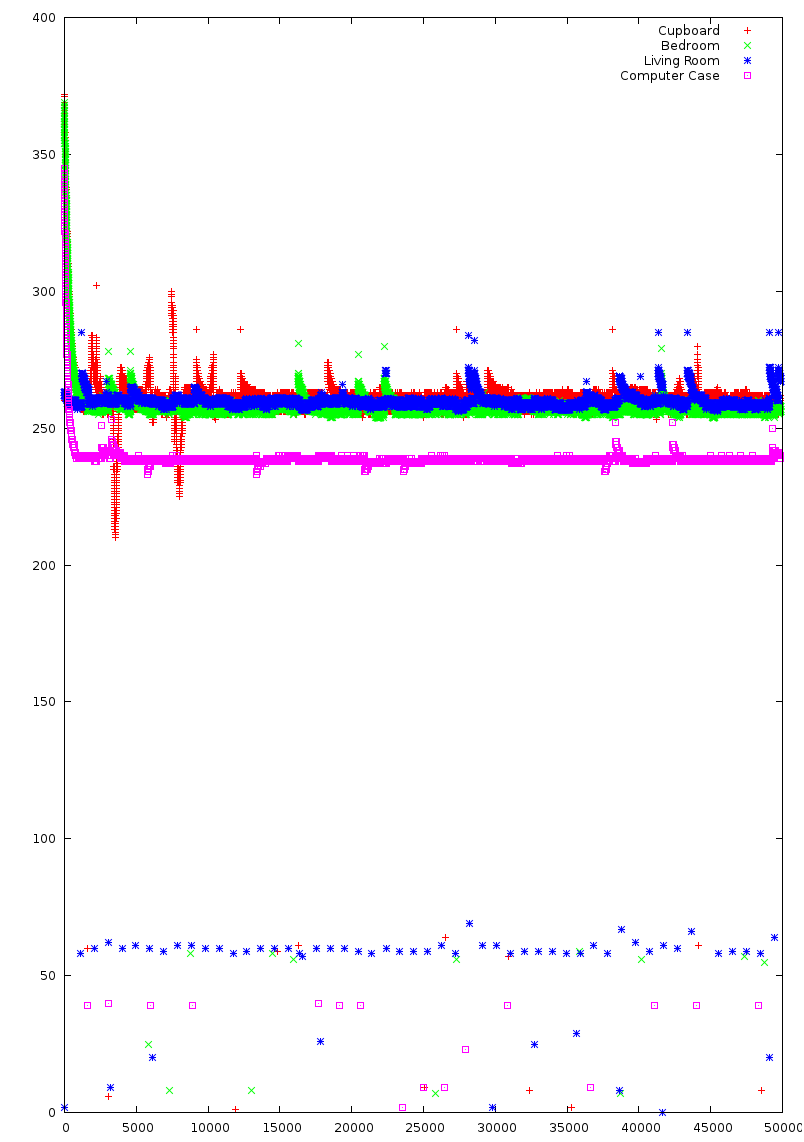
\includegraphics[width=0.7\columnwidth]{img/RoomTempOverlay.png}
  
  \caption{Readings from ard1 at Setting 0, in various places}
  \label{fig:ard3space}
\end{figure}


\begin{figure}[h!]
  \centering  
  \subfloat[200 readings from ard1 in setting 0]{
    \label{fig:ard1zoomroom}
    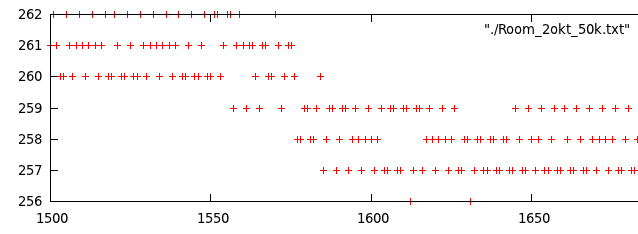
\includegraphics[width=0.7\columnwidth]{img/Room_1500-1700_zoom.png}
  }

  \subfloat[1000 readings from ard3 in setting 0]{
    \label{fig:ard3zoomroom}
    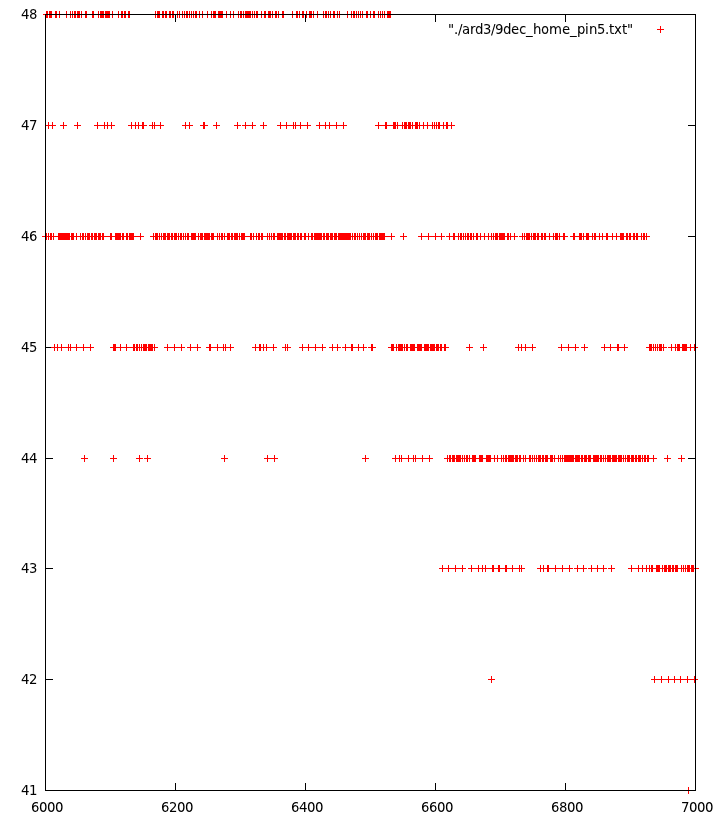
\includegraphics[width=0.7\columnwidth]{img/RoomZoom_9des.png}
  }

  \caption{Limited ranges of readings from \texttt{analogRead}}
  \label{fig:ardzoom}
\end{figure}

\begin{figure}[h!]
  \centering
  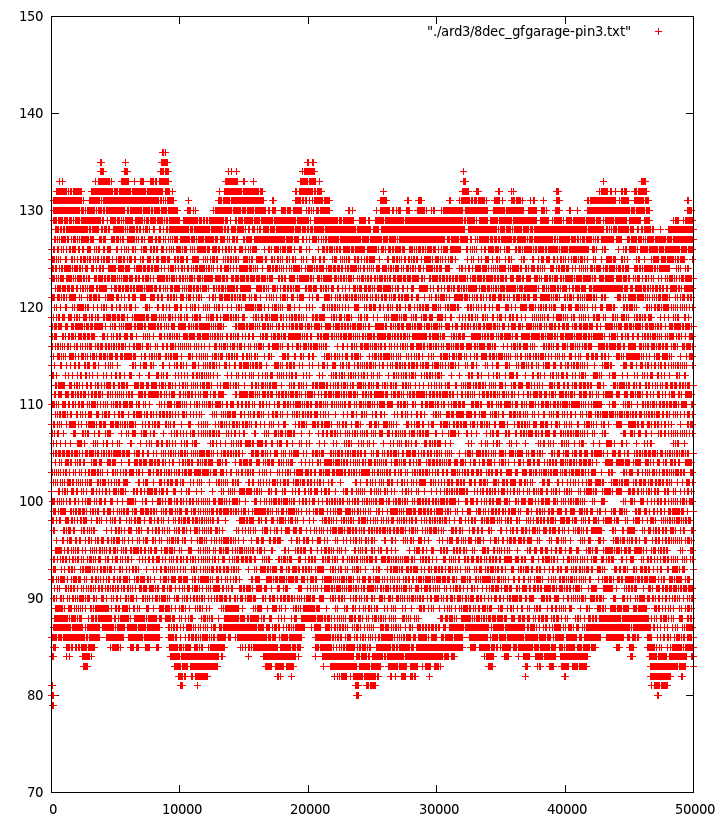
\includegraphics[width=0.7\columnwidth]{img/ard3gfgarage.png}
  \caption{Readings from ard3 taken in setting 1}
  \label{fig:gfgarageard3}
\end{figure}


\subsubsection{Effects of temperature}

Temperature is a key environmental factor. We see a much broader range of values when operating in heat or cold. The figures ~\ref{fig:ard1heat}, \ref{fig:ard1freezer} and\ref{fig:ard1fridge} show the output from \texttt{analogRead} in various temperature conditions of the extreme kinds. Note that ~\ref{fig:ard1freezer} only has 10000 values, as opposed to the 50000 values in all the other figures. This is because the Arduino simply stops working after a few minutes at $-11^\circ$C. Arduino have not released any information regarding operating temperatures but according to AVR the operating temperatures for the ATMega 328 microcontroller is $-40^\circ$C to $85^\circ$C \cite{atmegads}. One of our Arduino boards (ard1) broke after spending 4 hours in the freezer at $-12^\circ$C, so we conclude that some other component(s) on the board survive less cold than the microcontroller itself. 



\begin{figure}[H]
  \centering  
  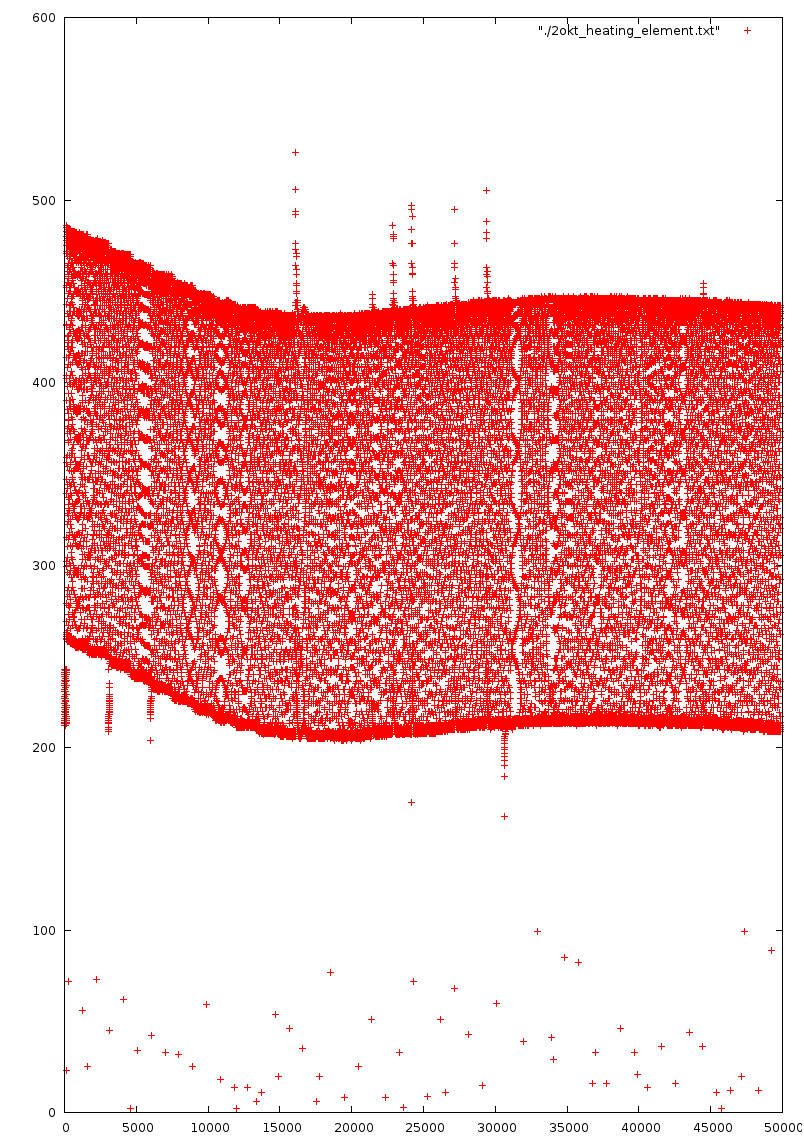
\includegraphics[width=0.7\columnwidth]{img/Heating50k.png}
  \caption{Readings on top of a hot heating element (approx. 40C) in setting 0}
  \label{fig:ard1heat}
\end{figure}

\begin{figure}[H]
  \centering  
  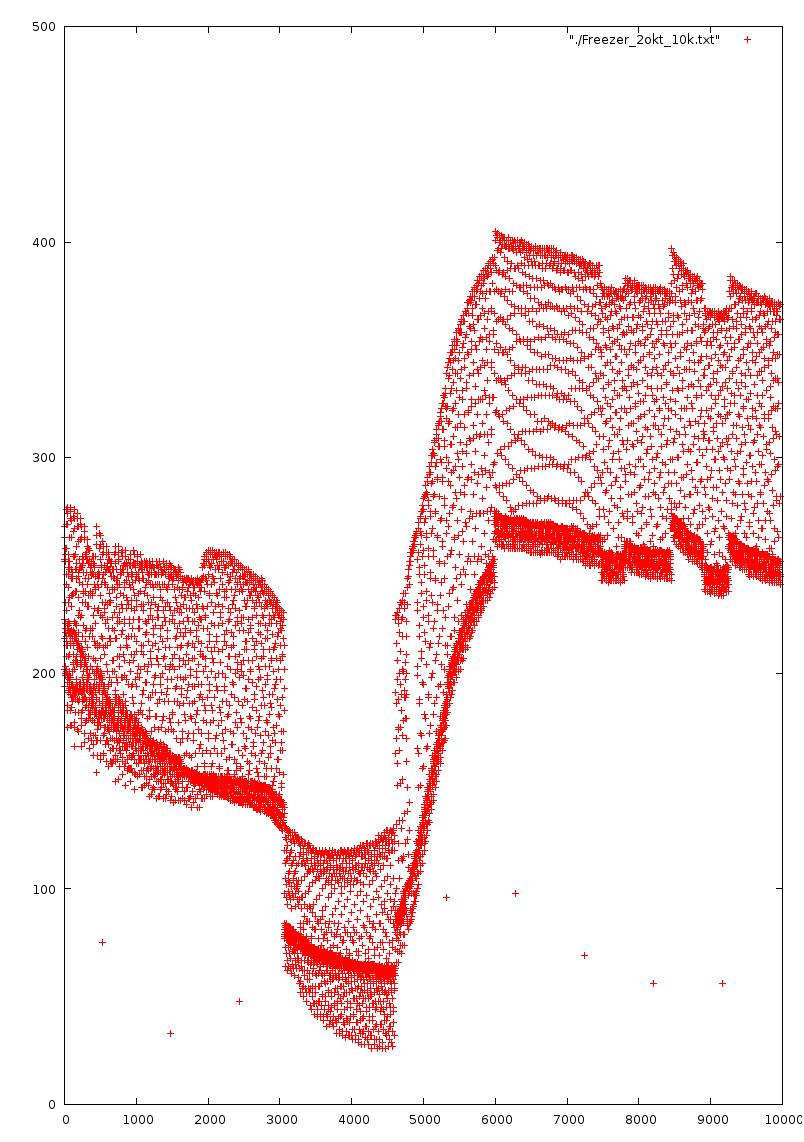
\includegraphics[width=0.7\columnwidth]{img/Freezer10k.png}
  \caption{Reading inside a freezer (approx. -11C) at setting 0}
  \label{fig:ard1freezer}
\end{figure}
  
\begin{figure}[H]
  \centering  
  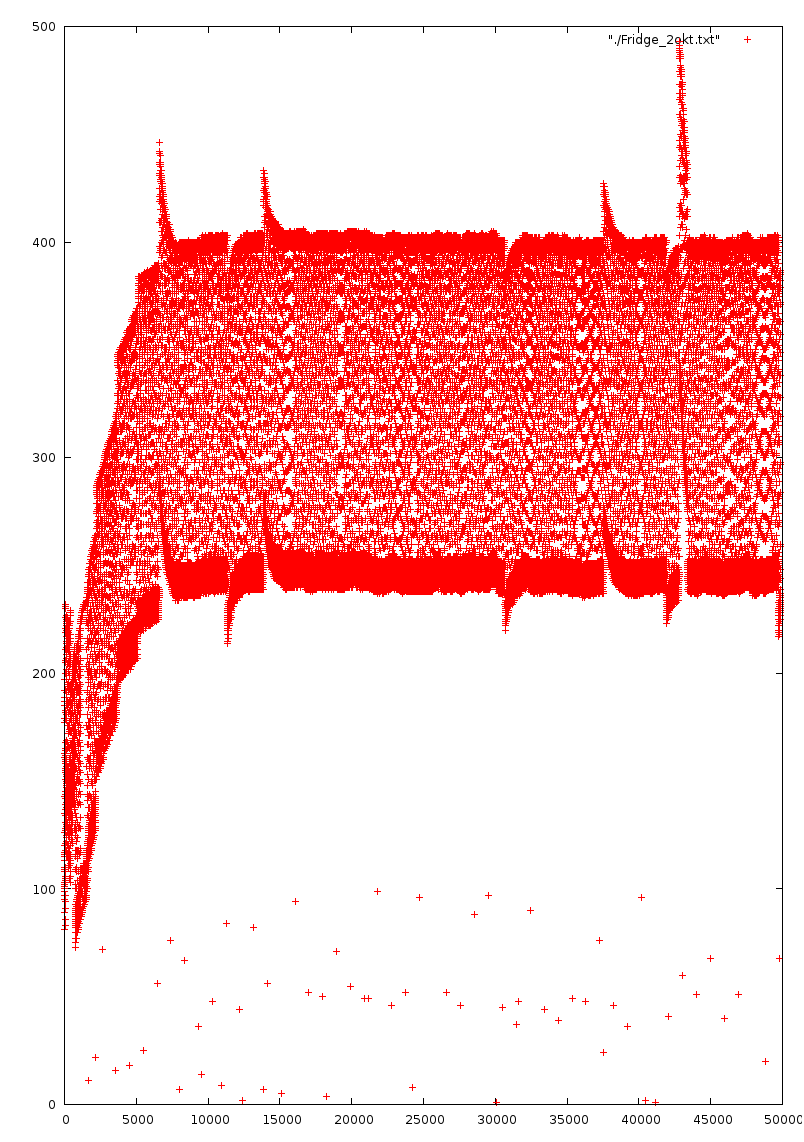
\includegraphics[width=0.7\columnwidth]{img/Fridge50k.png}
  \caption{Reading inside a fridge (approx. 1C) at setting 0}
  \label{fig:ard1fridge}
\end{figure}

\section{Breaking the Arduino as a RNG}

This section is twofold. We will both show that using the \texttt{analogRead} function to seed the \texttt{avr-libc} PRNG is a very bad idea and we also exhibit proof-of-concept code that finds such a seed value, given a sequence from the PRNG. 

\subsection{Refuting the claims made by Arduino}
\label{sec:refuting}


The Arduino Reference Manual\cite{ardref} states the following in the section about the \texttt{randomSeed} function. This claim is at the time of writing found in the manual, and is available via The Internet Archive\footnote{http://www.archive.org} at \url{http://web.archive.org/web/20110428064453/http://arduino.cc/en/Reference/RandomSeed}. The reference manual is only available online. 

\begin{quote}
``If it is important for a sequence of values generated by random() to differ, on subsequent executions of a sketch, use randomSeed() to initialize the random number generator with a fairly random input, such as analogRead() on an unconnected pin.''
\end{quote}

After having visually examined the raw output with the graphs in the section above, we clearly saw that the output is very likely non-random and not even ``fairly random'' as claimed. This would also explain the troubles we had in devising an algorithm that produces random bits. 

The first issue with \texttt{analogRead} is that it only returns 10-bit integers, since it reads from the 10-bit analog-to-digital converter on the Arduino board\footnote{See \url{http://arduino.cc/en/Reference/AnalogRead}}. It then follows trivially that if you use \texttt{analogRead} to seed the PRNG, there are only $2^{10} = 1024$ seed values for an adversary to explore. 

  \begin{figure}[h!]
    \centering  
    \subfloat[Sample from Ard3 taken in setting 0]{
      \label{fig:ard3home}
      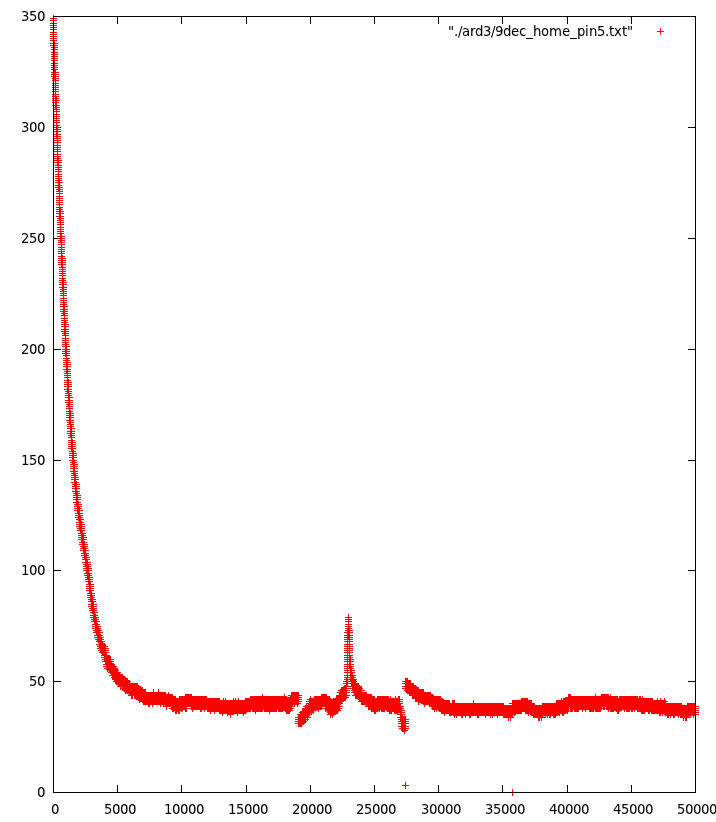
\includegraphics[width=0.7\columnwidth]{img/home-ard3-pin5.png}
    }

    \subfloat[Sample from Ard3 taken in setting 1]{
      \label{fig:ard3gfgaragepins}
      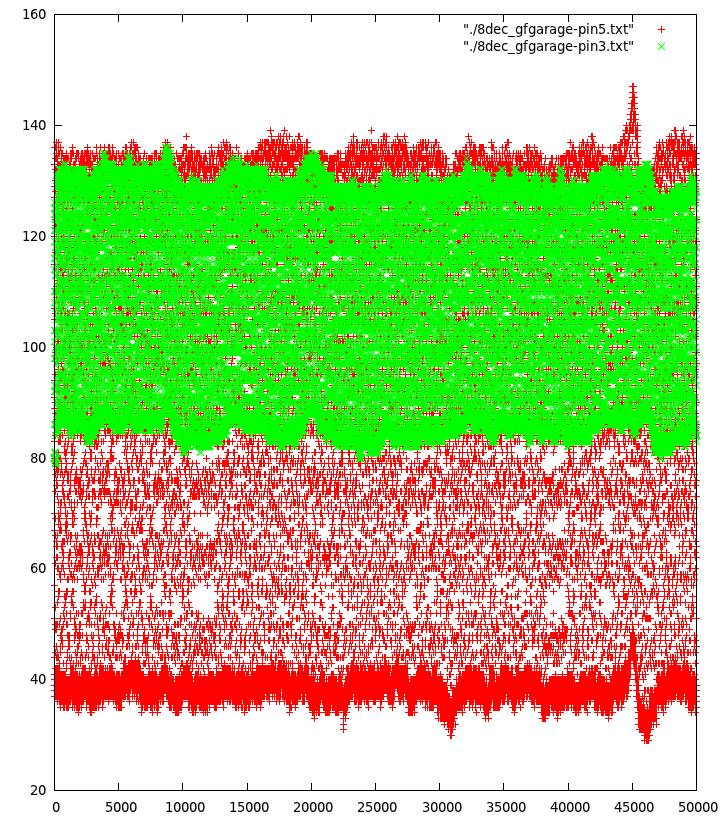
\includegraphics[width=0.7\columnwidth]{img/gfgarage-ard3-pin3_5.png}
    }

    \caption{Readings from our Arduino no. 3 on pins 3 (green) and pin 5 (red). NOTE: home pin3, show same scales}
    \label{fig:ard3}
        
  \end{figure}
 
As we can see from Figure~\ref{fig:ard3} there are only roughly 100 values that show up, but it is worth noting that using different pins give us different scopes of values. 

We exposed the output from \texttt{analogRead} to the same statistical tests as our \texttt{RAND} algorithms. In order to use the FIPS-bounds to measure against we needed 20 000 bits, or 2000 10-bit integers that we converted to binary. We state the null hypothesis

\[
H_0 = \text{The output from \texttt{analogRead} is "fairly random"}
\]

and show that the results are statistically significant and we can reject it as non-random. These are the average over three consecutive runs in setting 0. 

  \begin{table}[H]
    \begin{center}
      \begin{tabular}{| l | l | l | l |}
        \hline
        Statistical test & $X$ statistic & Accepted & Required $X$ interval \\
        \hline
        \hline
        \textbf{Monobit} & 903.847 & \textcolor{red}{\textbf{Rejected}} & $9.964 < X_1 < 10.346$  \\
        \textbf{Poker} & 3211.45 & \textcolor{red}{\textbf{Rejected}} & $1.03 < X_3 < 57.4$ \\
        \textbf{Runs} & 2812.81 & \textcolor{red}{\textbf{Rejected}} & Lengths of runs used \\
        \hline
      \end{tabular}
    \end{center}
    \caption{Results of the statistical test applied to \texttt{analogRead} output}
    \label{tab:analogreadtests}
  \end{table}

We see that all of the statistics are far off from the FIPS requirements so we can safely conclude that the null hypothesis $H_0$ is false and \texttt{analogRead} is not even ``fairly random''. 

We note that the observed bitrate for reading values directly from \texttt{analogRead} is 17531 bps\footnote{Baudrate 115200 bps}. 

\subsection{Finding the seed}
\label{sec:seedfind}

This limited range of possible values from \texttt{analogRead} cuts down on search time for the seed. As we have seen, there are only a few hundred values that show up most of the time, although these values may vary. We have designed proof-of-concept code\footnote{Implemented in the file \texttt{seedfind.py} in the Ardrand codebase} that given a sequence from the \texttt{avr-libc} (Arduino) PRNG, finds the seed --- given that is was chosen by use of \texttt{analogRead}. 

The \texttt{avr-libc} PRNG is a Linear congruential generator defined by the recurrence relation\footnote{Resides in \texttt{libc/stdlib/random.c} in avr-libc-1.7.1 and a Python implementation is found at \texttt{avrlibcrandom.py} in the Ardrand codebase}

\[
X_{n+1} \equiv 7^5 \cdot X_n \pmod{2^{31} -1}.
\]

In order to account for the diversity in values that the Arduino outputs in various settings, our implementation inputs either a text file of samples or can connect to an Arduino board and collect fresh samples. To provide the same interface, this is implemented by means of inherited classes in the code. 

Let $C$ denote the number of calls a program has made to the PRNG in order to generate a sequence $s$. Let $m$ be our best-guess or estimation of the unknown $C$. Our program inputs $s$ and $m$, as well as a sample source. It then builds a list of values in the range $[0, 1023]$, sorted by the frequency by which they appear in the given sample. Let $P$ denote this list of probability distributed values.

We then create one deque for each of the $1024$ values in P. Let $k$ be the length of the sequence $s$. For all $i \in P$ we create a deque with $k$ pseudo random integers derived from $i$ as a seed. Then we iterate over $P$ and generate $k+m$ integers for each deque (holding $k$ values at a time) until we find the sequence. 

Here is pseudo-code for our program. The functions \texttt{srandom} and \texttt{random} are the seeding function for the \texttt{avr-libc} PRNG and random function, respectively. 

\begin{lstlisting}[caption=Finding the seed]
def findseed(s, m, samplesource):
  k = len(s)
  lastk = [deque()]*1024

  P = buildProbDist(samplesource)

  # Expand all the deques by k elements from P[i] as seed
  for i in P:
    srandom(i)
    lastk[i] = deque([random() for _ in range(k)])
    # Did we receive a sequence derived directly from the seed?
    if lastk[i] == s:
      return i+

  while True:
    for i in P:
      for _ in range(m+k):
        srandom(lastk[i][-1])
        v = random()
        lastk[i].popfront()
        lastk[i].append(v)
        if lastk[i] == s:
          return i
\end{lstlisting}

This program has running bounds given by $\mathcal{O}(C)$, since it has a endless \texttt{while}-loop, its running time is not bounded by the $\mathcal{O}(m+k)$ loop, that is only an estimation or best-guess of how long it takes to find the correct seed. 

\subsubsection{Possible optimizations}

While this program runs reasonably fast in practice, one can think of optimizations of the code. Let $G$ a sorted list of observed values in the sample source. Then one variation of the \texttt{findseed} program might generate sequences from each value $g \in G$ as seed for some constant time $t$ before moving on to the unlikelier values that are in $P-G$, the unobserved values. Thus we would spend $t$ times more time on the likelier values. The while loop of this variation would look like

\begin{lstlisting}[caption=One possible optimization of the \texttt{findseed} program]
...
  while True:
    for i in G:
      for _ in range(t*(m+k)):
        expand(lastk[i])
        if lastk[i] == s:
          return i
    for i in P-G:
      for _ i range(m+k):
        expand(lastk[i])
         if lastk[i] == s:
           return i

def expand(que):
  srandom(que[-1])
  v = random()
  que.popfront()
  lastk[i].append(v)
\end{lstlisting}


\section{Conclusions}

\bibliography{ardrand}{}
\bibliographystyle{plain}


\end{document}

% Stuff to mention
% Switching from 9600 baudrate to the new one resulting in leastsignrand passing poker test
% Also resulted in SerialException
% How closely the algs miss the FIPS test
% Bitrates in 9600 vs new one
% Check other baudrates?

% Eftir að gera
%% Sýna graf frá einum Arduino þar sem lesið er frá öllum pinnum
%% Athgua hvort að ard3 sýni drop á skógarbraut. Taka gröf úr ard2 líka. Skoða ard1
%% Sýna munin á gildum í mismuandi herbergjum (fossahvarf vs skógarbraut)

% Athugasemdir til Ýmis:
%% Mig vantar að orða tengsl við Tsense einhversstaðar
%%% Tsense notaði einmitt aðferðina að lesa analogRead til að búa seed, koma því að
%% Eiga öll NIST security levels erindi í skýrsluna?
%% Ég set footnote á randomSeed referencið í introduction en myndi líka að þurfa að vitna í það í seinni kafla. Hvernig geri ég það snyrtilegast?